\begin{frame}[fragile]{7-Segment Anzeigen}
	\metroset{block=fill}
	\begin{block}{Können Zahlen zeigen}
		\begin{center}
			\sevensegnum[size=15mm]{2}%
			\hspace{1em}
			\sevensegnum[size=15mm]{0}%
			\hspace{1em}
			\sevensegnum[size=15mm]{2}%
			\hspace{1em}
			\sevensegnum[size=15mm]{5}%
		\end{center}
	\end{block}
	\pause
	\begin{block}{Zeigen manchmal wirres Zeugs}
		\begin{center}
			\sevenseg[size=15mm]{{0,0,0,1,0,0,0,}}%
			\hspace{1em}
			\sevenseg[size=15mm]{{0,1,0,0,1,0,0,}}%
			\hspace{1em}
			\sevenseg[size=15mm]{{1,1,0,1,1,1,1,}}%
			\hspace{1em}
			\sevenseg[size=15mm]{{1,0,1,1,0,0,0,}}%
		\end{center}
	\end{block}
\end{frame}

\begin{frame}{\only<2->{\xout}{Der Checker} \only<2->{Das Prädikat}}
	Wir brauchen einen \textit{Checker}:
	\Huge
	\begin{center}
		$
			\only<1,2>{P_{\text{Zahl}}\left(\sevensegnum{6}\right)}
			\only<3->{P_{\text{Zahl}}\left(\sevenseg{{1,0,1,1,0,0,0,}}\right)}
		$
	\end{center}
	\normalsize
	% todo
	\only<1>{Wenn wir in diesen \textit{Checker} (genannt Prädikat) eine Anzeige einsetzen, haben wir eine logische Aussage}
	\only<2-3>{
		\begin{tikzpicture}[overlay]
			\node[] at (5,.8) (base) {};
			\node[] at (2, -.4) (wahr) {
				\only<2>{\alert}{Wahr}, wenn eine Zahl zu sehen ist
				};
			\draw[->] (base) to (wahr);
			\only<3>{\node[] at (8, -.4) (wahr) {
				\alert{Falsch}, wenn keine Zahl zu sehen ist
				};
			\draw[->] (base) to (wahr);
			}
		\end{tikzpicture}
	}
\end{frame}

{\setbeamercolor{palette primary}{bg=ExColor}
\begin{frame}{Denkpause}
	Sind die folgenden Aussagen wahr oder falsch
	\metroset{block=fill}
	\begin{block}{Normal}
		\begin{itemize}
			\item $A_1$: $P_{\text{Zahl}}\left(\sevensegnum[]{7}\right)$ \only<2->{\hspace{1cm}wahr}
			\item $A_2$: $P_{\text{Zahl}}\left(\sevenseg[]{{0,1,0,0,1,0,1}}\right)$ \only<3->{\hspace{1cm}falsch}
			\item $A_3$: $P_{\text{Zahl}}\left(\sevensegnum[]{4}\right)$ \only<4->{\hspace{1cm}wahr}
			\item $A_4$: $P_{\text{Zahl}}\left(\sevenseg[]{{1,0,1,0,1,0,1}}\right)$ \only<5>{\hspace{1cm}falsch}
		\end{itemize}
	\end{block}
\end{frame}
}

\begin{frame}{Beispiel}
	Wie reparieren wir die Anzeige?
	\begin{center}
		\sevenseg[size=15mm]{{0,0,0,1,0,0,0,}}
		\hspace{1em}
		\sevenseg[size=15mm]{{0,1,0,0,1,0,0,}}
		\hspace{1em}
		\sevenseg[size=15mm]{{1,1,0,1,1,1,1,}}
		\hspace{1em}
		\sevenseg[size=15mm]{{1,0,1,1,0,0,0,}}
	\end{center}
\end{frame}

\begin{frame}{Beispiel}
	Wir brauchen eine Funktion, die Segmente einschaltet
	\Large
	\begin{center}
		$
			f_{\text{On}}\left(
			\sevenseg[size=10mm]{{1,0,0,1,0,0,1,}},
			\sevenseg[size=10mm]{{0,1,1,0,1,1,0,}}
			\right) =
			\sevenseg[size=10mm]{{1,1,1,1,1,1,1,}}
		$
	\end{center}
	\normalsize
	\only<3->{Wir brauchen eine weitere Funktion:
		\Large
		\begin{center}
			$
				f_{\text{On}}\left(
				\sevenseg[size=10mm]{{1,0,0,1,0,0,1,}},
				\sevenseg[size=10mm]{{0,1,1,0,1,1,0,}}
				\right) =
				\sevenseg[size=10mm]{{1,1,1,1,1,1,1,}}
			$
		\end{center}
		\normalsize
	}
	Reicht das?
	\begin{itemize}
		\item<2-> $f_{\text{On}}\left(\sevenseg{{0,0,0,1,0,0,0,}}, \sevenseg{{0,1,1,0,1,1,0,}}\right) = \sevensegnum{2}$
		\item<2-> $f_{\text{On}}\left(\sevenseg{{0,1,0,0,1,0,0,}}, \sevenseg{{0,1,1,0,1,1,0,}}\right) = \sevensegnum{2}$
		\item<2-> $f_{\text{On}}\left(\sevenseg{{1,1,0,1,1,1,1,}}, \sevenseg{{0,1,1,0,1,1,0,}}\right) = \sevensegnum{2}$
		\item<2-> $f_{\text{On}}\left(\sevenseg{{1,0,1,1,0,0,0,}}, \sevenseg{{0,1,1,0,1,1,0,}}\right) = \sevensegnum{2}$
	\end{itemize}
\end{frame}

\begin{frame}{Beispiel}
	Kombiniert mit unserem \textit{Checker}
	\Large
	\begin{center}
		$
			P_{\text{Zahl}}\left(f_{\text{On}}\left(
			\sevenseg[size=10mm]{{1,0,0,0,0,0,0,}},
			\sevenseg[size=10mm]{{0,1,1,0,0,0,0,}}
			\right)\right)
		$
	\end{center}
	\normalsize
	\pause
	Diese Aussage ist wahr
	\par
	\pause
	Allgemeiner:
\end{frame}

{\setbeamercolor{palette primary}{bg=ExColor}
\begin{frame}{Denkpause}
	Finde Anzeigen $x, y$, für die die Aussage stimmt
	\metroset{block=fill}
	\begin{block}{Normal}
		\begin{itemize}
			\item $P_{\text{Zahl}}\left(f_{\text{On}}\left(\sevenseg{{0,0,0,0,0,0,0,}}, x_1\right)\right)$
			\item $P_{\text{Zahl}}\left(f_{\text{Off}}\left(x_2, y_2\right)\right)$
			\item $P_{\text{Zahl}}\left(f_{\text{Off}}\left(x_3, \sevenseg{{0,1,1,0,0,0,0,0,}}\right)\right) \land P_{\text{Zahl}}\left(f_{\text{On}}\left(x_3, \sevenseg{{1,0,0,1,0,0,0,}}\right)\right)$
			\item $\lnot P_{\text{Zahl}}\left(f_{\text{On}}\left(f_{\text{On}}\left(\sevenseg{{0,0,0,0,0,0,0,}}, x_4\right), \sevenseg{{1,1,1,1,0,0,1,}}\right)\right)$
		\end{itemize}
	\end{block}
	Beweise ob die folgenden Aussagen wahr oder falsch sind
	\metroset{block=fill}
	\begin{block}{Etwas schwerer}
		\begin{itemize}
			\item $A_5$: $\forall x : P_{\text{Zahl}}\left(f_{\text{On}}\left(x, \sevenseg{{1,1,1,1,1,1,1,1,}}\right)\right)$
			\item $A_6$: $\forall x : P_{\text{Zahl}}\left(f_{\text{On}}\left(\right)\right)$
		\end{itemize}
	\end{block}
\end{frame}
}